
%Some information may be repeated from Lab4 as we are unsure on 100% of its contents
\section{Objectives}
By the end of this laboratory assignment, students are expected to learn how to 

\begin{itemize}

\item implement a conventional feedback controller  using a digital computer,
  
\item apply feedback control techniques for controlling rotational speed of a DC motor, and 
  
\item improve performance of DC motor control system by varying different parameters. 
 
  
\end{itemize}


\section{Parts}
\label{sec:partsDC_MotorControl1}
The main parts needed to conduct this laboratory experiment are: %
%
\begin{inparaenum}[a)]
% \item Breadboard,
\item BeagleBone Blue (BBBlue) embedded computer,
\item One Micro-USB cable, 
\item Laptop computer, 
\item One 2-pin JST ZH connector,
\item One Pittmann DC motor,
\item One IN4004 Diode\footnote{\href{http://www.onsemi.com/pub/Collateral/1N4001-D.PDF}{http://www.onsemi.com/pub/Collateral/1N4001-D.PDF}},
\item Power supply,
\item Two 2N2222A transistors\footnote{\href{http://www.st.com/web/en/resource/technical/document/datasheet/CD00003223.pdf}{http://www.st.com/web/en/resource/technical/document/datasheet/CD00003223.pdf}},
\item Two $10~[\si{\kilo\ohm}]$ resistors,
\item Two $100~[\si{\kilo\ohm}]$ resistors,
\item Two $1~[\si{\kilo\ohm}]$ resistors,
\item Oscilloscope, and 
\item Function generator.
\end{inparaenum}


% \section{Software}
% \begin{enumerate}
%     \item WinSCP
%     \item PuTTY
% \end{enumerate}



\section{Introduction}
\label{sec:introductionPID}
This laboratory assignment follows the setup conducted in Experiment~\ref{chap:dcMotorBBBlue} to control the rotational speed of a DC motor, \textit{i.e.,~} the motor shaft is supposed to rotate at a desired angular speed commanded by a user. There are many control strategies available for performing such a control task for a DC motor. Here, a conventional Proportional-Integral-Derivative (PID) control sheme will be used. The PID control strategy will be employed to demonstrate its performance in controlling the speed of  a DC motor by  conducting computer simulations and experiments using an embedded computer (BBBlue single-board computer, for example). The circuit shown in Figure~\ref{fig:rotaryEncoderInterface}  used to interface a Pittmann DC motor kit (see Figure~\ref{fig:pittmanDC-MotorKit}).    




\section{PID Controller Design}
\label{sec:pidControllerDesign}

Under no-load condition, let us consider a permanent-magnet  brushed DC motor shown in Figure~\ref{fig:pittmanDC-MotorKit}. Its input is the applied voltage, $V_a(t),$ across the motor $+/-$ terminals and output is the rotational speed (in RPM), $\omega_{\mathrm{shaft}}(t),$ of the motor shaft at time $t\ge 0$ with gear reduction ratio of $N:1.$ The block diagram showing the input and output relationship of the DC motor is shown in Figure~\ref{fig:dcMotorElecMechNoLoad}. %       
%
\begin{figure}
  \centering
    \fcolorbox{white}{gray!15}{
  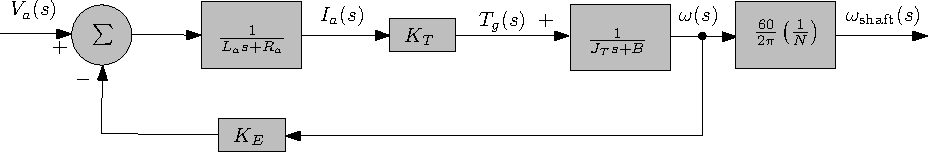
\includegraphics[width=0.6\textwidth]{figs/ipe/dcMotorElecMechNoLoad}}
\caption{Block diagram representation showing relationship between the applied voltage, $V_a,$ at the motor $+/-$ terminals and  the shaft speed $\omega_{\mathrm{shaft}}$ (in RPM).}
\label{fig:dcMotorElecMechNoLoad}
\end{figure}
%
Clearly, the transfer function of the DC motor model shown in Figure~\ref{fig:dcMotorElecMechNoLoad} is given by %
%
\begin{align}
  \label{eq:GM1}
    G_M(s) = \frac{\omega_{\mathrm{shaft}}(s)}{V_a(s)} = \left(\frac{60}{2\pi N}\right)\frac{K_T}{\left(L_as + R_a\right)\left(J_Ts + B\right) + K_TK_E}.
\end{align}
%
Let us design a PID controller for the DC motor modeled by the transfer function~\eqref{eq:GM1} so that the motor shaft speed $\omega_{\mathrm{shaft}}(t)$ follows the reference speed (given), $\omega^{\mathrm{ref}}$ at time $t\to\infty.$ Figure~\ref{fig:dcMotorElecMechNoLoadControl} shows the overall closed--loop (voltage) control system of a DC motor, where $U(s)$ and $E(s)$ are the Laplace transformation of the control signal $u(t)$ and the speed error signal, $e(t),$ respectively. %
%
\begin{figure}
  \centering
    \fcolorbox{white}{gray!15}{
  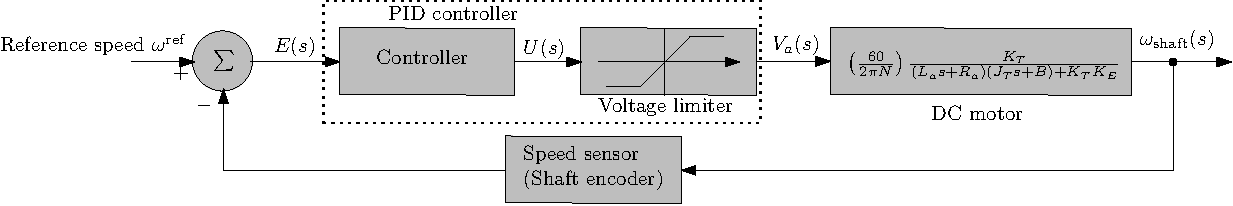
\includegraphics[width=0.6\textwidth]{figs/ipe/dcMotorElecMechNoLoadControl}}
\caption{Closed-loop PID control structure of a DC motor.}
\label{fig:dcMotorElecMechNoLoadControl}
\end{figure}
%

The controller takes error $e(t)$ as the input and gives the control signal $u(t)$ as an output. The control signal $u(t)$ is then passed through a voltage limiter so that $V_a\in[0,V_{\mathrm{ref}}],$ is applied at the motor $+/-$ terminals, where $V_{\mathrm{ref}}$ is the maximum reference voltage of the motor. A conventional PID controller defined by %
%
\begin{align}
  u(t) = K_pe(t) + K_i\int_0^te(t)\mathrm{dt} + K_d\frac{\mathrm{d}e(t)}{\mathrm{dt}},
  \label{eq:PID-Time}
\end{align}
%
can be implemented using a digital (embedded) computer, where $K_p,~K_i,~K_d\ge 0$ are the parameters of the controller that are tuned to determine the performance of the output.  The Laplace transformation of model~\eqref{eq:PID-Time} is simply %
%
\begin{align}
  U(s) = \left[K_p+\frac{K_i}{s} + K_d s\right]E(s).
  \label{eq:PID-Laplace}
\end{align}
%
The shaft speed of the motor can be measured using a quadrature encoder interfaced with the digital computer.   The PID controller can also be designed to produce pulse width modulation (PWM)  signals that drive the motor using a PWM drive. The block diagram that implements such a controller is shown in Figure~\ref{fig:dcMotorElecMechNoLoadPWM-Control}, where the output of the controller is now the duty cycle $\rho(t),$ that takes the value between $0$ and $1.$ Note that  $\rho(t) = 0$ and  $\rho(t) = 1$ corresponds to $0\%$ and $100\%$ duty cycles, respectively. %     
%
\begin{figure}
  \centering
    \fcolorbox{white}{gray!15}{
  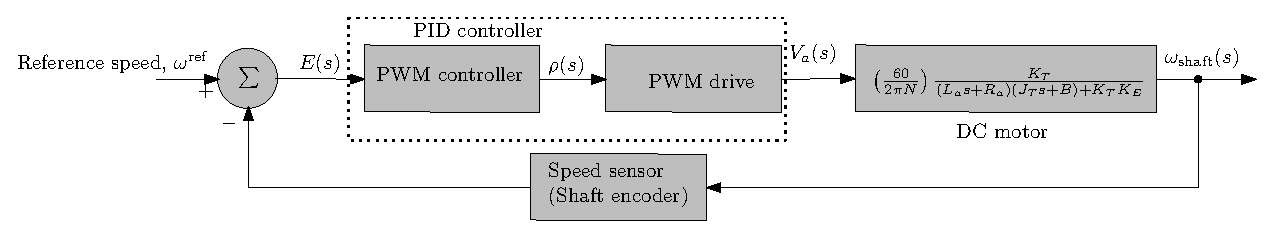
\includegraphics[width=0.6\textwidth]{figs/ipe/dcMotorElecMechNoLoadPWM-Control}}
\caption{Closed-loop PWM control structure of a DC motor.}
\label{fig:dcMotorElecMechNoLoadPWM-Control}
\end{figure}
%
The control signal $\rho(t)$ is then passed through a PWM drive circuit to drive the motor with appropriate volage and current for achieving desired rotational speed. %
%

\section{Prelab}
\label{sec:prelabDC-MotorControl1}
Before you start working on the prelab, it is important to read the theoretical background of a PID control strategy discussed in section~\ref{sec:pidControllerDesign}. Furthermore, the values of the motor parameters should be recorded from the datasheet of the Pittman DC motor\footnote{See the Pittman DC motor datasheet at \href{http://www.precisionmotorworks.com/pdf/Pittman_GM87xx.web.pdf}{http://www.precisionmotorworks.com/pdf/Pittman\_GM87xx.web.pdf} [Note: highlighted values in the datasheet may not correspond to the motor that is used in this laboratory experiment. Therefore, choose the correct values of the DC motor used for this laboratory experiment]}. %The datasheet of the DC motor used in this experiment can be found at %
%
% \url{http://www.precisionmotorworks.com/pdf/Pittman_GM87xx.web.pdf} %or %
% %
% \url{http://ee.bradley.edu/projects/proj2003/cntrlwrk/gm9000_pittman.pdf}
% %
%
\begin{prelab}[DC motor control using Simulink]{prelab:DC-MotorControlSimulink}
As mentioned, this laboratory experiment deals with a permanent magnet brushed DC motor (see its schematic diagram shown in Figure~\ref{fig:DC-MotorSchematic}). Therefore, the motor's field intensity is fixed. 
%
\begin{enumerate}
\item Record the values of parameters from the motor's datasheet in the table below.

  \begin{center}
    \begin{tabular}{c|l|l|l}
      \toprule
      Symbol & Description & Value & Unit\\
      \toprule
      $B$&Viscous damping coefficient&$\ldots$&$[\si{\newton\cdot\meter\per(\radian\per\second)}]$\\
      $J_m$&Motor shaft's moment of inertia&$\ldots$&$[\si{\kilogram\meter}^2]$\\      
      $K_E$&Back-emf constant &$\ldots$&$[\si{\volt\per(\radian\per\second)}]$\\
      $K_T$&Motor torque constant &$\ldots$&$[\si{\newton\meter\per\ampere}]$\\
      $L_a$&Armature inductance &$\ldots$&$[\si{\henry}]$\\            
      $R_a$&Armature resistance &$\ldots$&$[\si{\ohm}]$\\
      $N:1$&Gear reduction ratio &$\ldots$&N/A\\      
      \bottomrule
    \end{tabular}    
  \end{center}
% \item Determine the values of the electrical $(\tau_E)$ and mechanical $(\tau_M)$ time constants.
% %
%   \begin{center}
%     \begin{tabular}{c|c|c}
%       \toprule
%       Time constant &  Computed & Datasheet value\\
%       \toprule
%       $\tau_E$ & $\ldots$ & $\ldots$\\
%       $\tau_M$ & $\ldots$ & $\ldots$\\
%       \bottomrule
%     \end{tabular}    
%   \end{center}
\item  Use Simulink to model the PID controller with performance parameters $K_p = 0.1,$ $K_i = 9,$ and $K_d = 10^{-6}$ and then implement the closed-loop motor control system given by the block diagram shown in Figure~\ref{fig:dcMotorElecMechNoLoadControl}, where the motor is operating at no-load conditions and the friction torques are assumed to be negligible, \textit{i.e.,~}$T_L + T_f +T_{\mathrm{gr}} = 0,$ and the sum of mass moments of inertia of the motor $J_T$ is same as the motor's rotor inertia $J_m$ (\textit{i.e.,} $J_T=J_m).$
  
\item Run the Simulink model constructed in the previous step for $0.2~[\second]$ and then use MATLAB to plot the motor shaft speed $\omega_{\mathrm{shaft}}(t)$ versus time $t$ and motor applied voltage  $V_a(t)$ versus time $t$ for the reference speed    %
  \begin{itemize}
  \item $\omega^{\mathrm{ref}} = 520~\mathrm{RPM},$
  \item $\omega^{\mathrm{ref}} = 400~\mathrm{RPM},$ and 
  \item $\omega^{\mathrm{ref}} = 330~\mathrm{RPM}.$    
  \end{itemize}

  [Note: You are to provide six plots in total (two plots  for each reference speed $\omega_{\mathrm{shaft}})$ ]
\end{enumerate}

\end{prelab}
%




\begin{prelab}[PWM control of DC motor]
  ~

Draw a flowchart (not handwritten!)  of the algorithm that implements the PWM control system shown in Figure~\ref{fig:dcMotorElecMechNoLoadPWM-Control} so that the motor shaft speed follows the reference speed $\omega^{\mathrm{ref}}$ entered by a user. 
\end{prelab}

\section{Laboratory Work}

You are to implement a PWM controller shown in Figure~\ref{fig:dcMotorElecMechNoLoadPWM-Control} using BBBlue embedded computer.  




\begin{enumerate}

\item Connect a $2$-pin JST ZH connector with the DC motor driver channel $\#1.$
  
\item Design and construct the output signal conditioning circuit shown in the block diagram of Figure~\ref{fig:dcMotorBBBlueBD}.

\item Connect a 2-cell lithium battery pack (make sure to check for enough charge in the battery) to the robotics cape embedded into the BBBlue computer.
  
\item To construct the circuit shown in Figure~\ref{fig:rotaryEncoderInterface}, measure the resistance of the $1~[\kilo\ohm],$ $10~[\kilo\ohm],$ $100~[\kilo\ohm]$  resistors $(R_1,R_2,R_3,R_4,R_5$ and $R_6).$ Then, complete the following table.

  \begin{center}
    \begin{tabular}{c|l|l}
      \toprule
      Quantity &  Ideal~$[\kilo\ohm]$ & Measured~$[\kilo\ohm]$\\
      \toprule
      $R_1$ & $1$ & $\ldots$\\   %|| R_1 =
      $R_2$ & $100$ & $\ldots$\\   %|| R_2 =       
      $R_3$ & $10$ & $\ldots$\\   %|| R_3 =
      $R_4$ & $1$ & $\ldots$\\   %|| R_4 =
      $R_5$ & $100$ & $\ldots$\\   %|| R_3 =
      $R_6$ & $1$ & $\ldots$\\   %|| R_4 =             
      \bottomrule
    \end{tabular}    
  \end{center}
  
\item Construct the circuit shown in Figure~\ref{fig:rotaryEncoderInterface} using the components measured in the previous step.

 
\item Write a program for your BBBlue  that implements the PWM control strategy shown in Figure~\ref{fig:dcMotorElecMechNoLoadPWM-Control} so that the measured shaft speed follows the reference speed $\omega^{\mathrm{ref}} = 80~[\mathrm{RPM}]$ (given).
  



\item Comment on any discrepancy found between the computed and the experimental (measured) values of the no-load speeds  and and no-load currents. 

  
\end{enumerate}







%%% Local Variables:
%%% mode: latex
%%% TeX-master: "../../labHandoutMechatronics-V1"
%%% End:
